\section{The Enumeration Algorithm}

\begin{frame}{Permutation Representation of Subgraphs}

\begin{lemma}
Any subgraph $H$ of $\CGrid$ with $|V(H)| = n$ can be uniquely identified as a permutation of $[n]$, denoted $\pi(H)$.
\end{lemma}

\begin{proof}<2->
Since $H \subseteq \CGrid$, each vertex has distinct $x,y$ coordinates. Name vertex $i$ by its rank sorting by $x + \frac{y}{n}$. Denote $\pi_i$ by the rank of vertex $i$ sorted by $y + \frac{x}{n}$. 

\vspace{0.5cm}

Conversely, given a permutation $\pi \in S_n$, construct vertices $(i, \pi_i)$ for $i=1,\dots,n$. This produces a subgraph of $\CGrid$ with $n$ vertices.

\vspace{0.5cm}

These are inverses of each other.
\end{proof}

\end{frame}

\begin{frame}{Example Permutation Representation}

\begin{example}
The following subgraph $H$ has $\pi(H) = (2,1,4,3)$, since the leftmost vertex is 2nd lowest in $y$ order, and so on.
\end{example}

\vspace{0.5cm}

\centering
\begin{tikzpicture}[
    scale=1.3,
    dot/.style={circle, inner sep=1.5pt},
    faintdot/.style={dot, fill=black!25},
    sel/.style={dot, fill=black},
    faintedge/.style={line width=0.55pt, draw=black!25},
    seledge/.style={line width=0.85pt, draw=black},
    lab/.style={draw=none, fill=none, inner sep=0pt, font=\small},
]

\begin{scope}[xshift=0cm]
    % vertices
    \foreach \x in {1,2,3}{
    \foreach \y in {1,2,3}{
        \node[faintdot] (L-\x-\y) at (\x,\y) {};
    }
    }

    % select vertices (2,1), (1,2), (2,3), (3,2)
    \node[sel] (Lsel-2-1) at (2,1) {};
    \node[sel] (Lsel-1-2) at (1,2) {};
    \node[sel] (Lsel-2-3) at (2,3) {};
    \node[sel] (Lsel-3-2) at (3,2) {};

    % (faint) edges of CGrid_{3x3} copied from your reference
    \draw[faintedge] (L-1-1) -- (L-1-2);
    \draw[faintedge] (L-1-1) -- (L-2-1);
    \draw[faintedge] (L-1-1) -- (L-2-2);
    \draw[faintedge] (L-1-1) -- (L-2-3);
    \draw[faintedge] (L-1-1) -- (L-3-2);

    \draw[faintedge] (L-1-2) -- (L-1-3);
    \draw[faintedge] (L-1-2) -- (L-2-2);
    \draw[faintedge] (L-1-2) -- (L-2-3);

    \draw[faintedge] (L-1-3) -- (L-2-3);

    \draw[faintedge] (L-2-1) -- (L-2-2);
    \draw[faintedge] (L-2-1) -- (L-3-1);
    \draw[faintedge] (L-2-1) -- (L-3-2);

    \draw[faintedge] (L-2-2) -- (L-2-3);
    \draw[faintedge] (L-2-2) -- (L-3-2);

    \draw[faintedge] (L-2-3) -- (L-3-3);
    \draw[faintedge] (L-3-1) -- (L-3-2);
    \draw[faintedge] (L-3-2) -- (L-3-3);

    \draw[faintedge] (L-1-1) to[bend left=20] (L-1-3);
    \draw[faintedge] (L-2-1) to[bend left=20] (L-2-3);
    \draw[faintedge] (L-3-1) to[bend left=20] (L-3-3);

    \draw[faintedge] (L-1-1) to[bend right=20] (L-3-1);
    \draw[faintedge] (L-1-2) to[bend right=20] (L-3-2);

    \draw[faintedge] (L-1-1) to[bend right=20] (L-3-3);
    \draw[faintedge] (L-1-2) to[bend right=20] (L-3-3);
    \draw[faintedge] (L-1-3) to[bend right=20] (L-3-3);

    \draw[faintedge] (L-2-1) to[bend right=20] (L-3-3);
    \draw[faintedge] (L-2-2) to[bend right=20] (L-3-3);

    % chosen subgraph edges among the 4 chosen vertices
    \draw[seledge] (L-2-1) -- (L-3-2);
    \draw[seledge] (L-2-1) -- (L-2-3);
    \draw[seledge] (L-1-2) -- (L-3-2); 
    \draw[seledge] (L-1-2) -- (L-2-3);

    % corner labels (optional)
    \node[lab, anchor=east] at ($(L-1-1)+(-0.25,0)$) {$(1,1)$};
    \node[lab, anchor=east] at ($(L-1-3)+(-0.25,0)$) {$(1,3)$};
    \node[lab, anchor=west] at ($(L-3-1)+(0.25,0)$) {$(3,1)$};
    \node[lab, anchor=west] at ($(L-3-3)+(0.25,0)$) {$(3,3)$};
\end{scope}

% ---------------------------
% Arrow to sheared grid
% ---------------------------
\draw[->,thick] (3.5,2) to (4.5,2);

% ---------------------------
% Helper: middle grid (shear/shift y by 0.2*(x-1))
% (x,y) -> (x, y + 0.2*(x-1))
% ---------------------------
\begin{scope}[xshift=4cm]
    % vertices
    \foreach \x in {1,2,3}{
    \foreach \y in {1,2,3}{
        \pgfmathsetmacro{\dx}{0.2*(\y-1)} % shift x depending on y
        \pgfmathsetmacro{\dy}{0.2*(\x-1)} % shift y depending on x
        \node[faintdot] (M-\x-\y) at (\x+\dx,\y+\dy) {};
    }
    }

    % select vertices
    \node[sel] (Msel-2-1) at (2,1+0.2) {};
    \node[sel] (Msel-1-2) at (1+0.2,2) {};
    \node[sel] (Msel-2-3) at (2+0.4,3+0.2) {};
    \node[sel] (Msel-3-2) at (3+0.2,2+0.4) {};

    % faint edges: same adjacency, just using shifted coordinates
    \draw[faintedge] (M-1-1) -- (M-1-2);
    \draw[faintedge] (M-1-1) -- (M-2-1);
    \draw[faintedge] (M-1-1) -- (M-2-2);
    \draw[faintedge] (M-1-1) -- (M-2-3);
    \draw[faintedge] (M-1-1) -- (M-3-2);

    \draw[faintedge] (M-1-2) -- (M-1-3);
    \draw[faintedge] (M-1-2) -- (M-2-2);
    \draw[faintedge] (M-1-2) -- (M-2-3);

    \draw[faintedge] (M-1-3) -- (M-2-3);

    \draw[faintedge] (M-2-1) -- (M-2-2);
    \draw[faintedge] (M-2-1) -- (M-3-1);
    \draw[faintedge] (M-2-1) -- (M-3-2);

    \draw[faintedge] (M-2-2) -- (M-2-3);
    \draw[faintedge] (M-2-2) -- (M-3-2);

    \draw[faintedge] (M-2-3) -- (M-3-3);
    \draw[faintedge] (M-3-1) -- (M-3-2);
    \draw[faintedge] (M-3-2) -- (M-3-3);

    \draw[faintedge] (M-1-1) to[bend left=20] (M-1-3);
    \draw[faintedge] (M-2-1) to[bend left=20] (M-2-3);
    \draw[faintedge] (M-3-1) to[bend left=20] (M-3-3);

    \draw[faintedge] (M-1-1) to[bend right=20] (M-3-1);
    \draw[faintedge] (M-1-2) to[bend right=20] (M-3-2);

    \draw[faintedge] (M-1-1) to[bend right=20] (M-3-3);
    \draw[faintedge] (M-1-2) to[bend right=20] (M-3-3);
    \draw[faintedge] (M-1-3) to[bend right=20] (M-3-3);

    \draw[faintedge] (M-2-1) to[bend right=20] (M-3-3);
    \draw[faintedge] (M-2-2) to[bend right=20] (M-3-3);

    % chosen subgraph edges (same adjacency)
    \draw[seledge] (M-2-1) -- (M-3-2);
    \draw[seledge] (M-2-1) -- (M-2-3);
    \draw[seledge] (M-1-2) -- (M-3-2); 
    \draw[seledge] (M-1-2) -- (M-2-3);

    % corner labels (optional, now reflecting shear)
    \node[lab, anchor=east] at ($(M-1-1)+(-0.25,0)$) {$(1,1)$};
    \node[lab, anchor=east] at ($(M-1-3)+(-0.25,0)$) {$(1.2,3)$};
    \node[lab, anchor=west] at ($(M-3-1)+(0.25,0)$) {$(3,1.2)$};
    \node[lab, anchor=west] at ($(M-3-3)+(0.25,0)$) {$(3.3,3.3)$};
\end{scope}

\end{tikzpicture}

\end{frame}

\begin{frame}{The Enumeration Algorithm}

\begin{lemma}
Let $H$ be a subgraph with $|V(H)| = O(n)$ and $|E(H)| = O(n)$. Using a Fenwick tree, we can construct the degree sequence of $H$ from $\pi(H)$ in two passes of $O(n \log n)$ time.

\vspace{0.2cm}

\only<2->{
In the {\color{red} first pass}, construct the {\color{red} backward degree}, i.e. $\forall j < i$, find $\pi_i > \pi_j$. In the {\color{blue} second pass}, run the algorithm on $\pi(H)$ reversed to get the {\color{blue} forward degree}, i.e. $\forall j > i$, find $\pi_i < \pi_j$. 
\vspace{0.2cm}

The sum of both is the degree sequence.
}
\end{lemma}

\begin{example}<2->
\vspace{-0.5cm}
\[
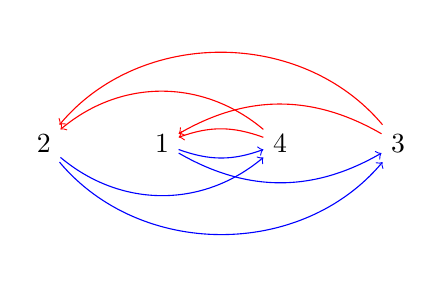
\begin{tikzpicture}[scale=1.5]
	\node (n1) at (0,0) {$2$};
	\node (n2) at (1,0) {$1$};
	\node (n3) at (2,0) {$4$};
	\node (n4) at (3,0) {$3$};

	\draw[->,color=blue] (n1) to[bend right=40] (n3);
	\draw[->,color=blue] (n1) to[bend right=50] (n4);
	\draw[->,color=blue] (n2) to[bend right=20] (n3);
	\draw[->,color=blue] (n2) to[bend right=30] (n4);

    \draw[->,color=red] (n3) to[bend right=40] (n1);
	\draw[->,color=red] (n3) to[bend right=20] (n2);
	\draw[->,color=red] (n4) to[bend right=50] (n1);
	\draw[->,color=red] (n4) to[bend right=30] (n2);


\end{tikzpicture}
\]
\end{example}

\end{frame}

\begin{frame}{The Enumeration Algorithm cont'd}

\begin{lemma}
Without even completing the {\color{red} first pass}, we can identify if $H$, $|V(H)| = n$, has more than $c = O(n)$ edges. By setting a corresponding minimum, we can enumerate all $H$ with $|V(H)| \in [b,c]$ with $O(n \log n)$ processing for each $H$.
\end{lemma}

\begin{example}
\vspace{-0.5cm}
\[
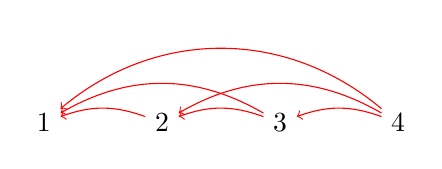
\begin{tikzpicture}[scale=1.5]
	\node (n1) at (0,0) {$1$};
	\node (n2) at (1,0) {$2$};
	\node (n3) at (2,0) {$3$};
	\node (n4) at (3,0) {$4$};

	\draw[<-,color=red] (n1) to[bend left=20] (n2);
    \draw[<-,color=red] (n1) to[bend left=30] (n3);
	\draw[<-,color=red] (n1) to[bend left=40] (n4);

	\draw[<-,color=red] (n2) to[bend left=20] (n3);
	\draw[<-,color=red] (n2) to[bend left=30] (n4);

	\draw[<-,color=red] (n3) to[bend left=20] (n4);
\end{tikzpicture}
\]
\end{example}

\end{frame}

\begin{frame}{The Enumeration Algorithm cont'd}

\begin{theorem}
Given an $n \in \mathbb{N}$, we can obtain a (small) set $H$ with
\begin{itemize}
    \item $|V(H)| = n$
    \item at least the number of edges in the target $\Grid$
    \item at most $k$ additional edges compared to the target $\Grid$
    \item degree sequence at least the degree sequence of target $\Grid$
    \item (some others)
\end{itemize}
with $O(n \log n)$ processing for each $H$.
\end{theorem}

\end{frame}

\begin{frame}{Recall: Which grids are subgraphs?}

\begin{theorem}
$\Grid_{k \times n}$ is not a subgraph of $\CGrid$ for $k > 2$. For $k = 3$, the minimum is 2 additional edges.
\end{theorem}

\begin{center}
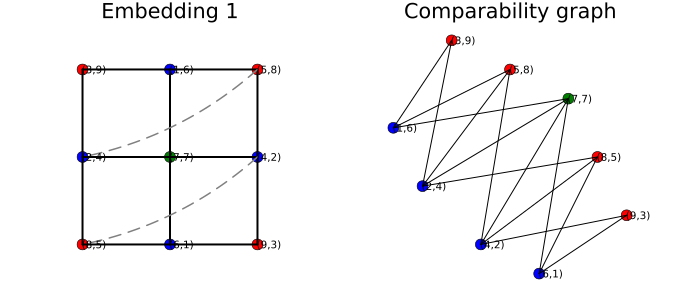
\includegraphics[width=\textwidth]{media/6-4-9-2-8-1-7-5-3.png}
\end{center}

\end{frame}

